\chapter{Clusters}
\label{chapter:clusters}

Clusters are aggregations of atoms or molecules connected via non-covalent
bonds such as van der Waals interaction, hydrogen bonds or metallic bonding.
They are interesting
because their properties lie in between the properties of
atoms and molecules on the one hand and macroscopic solid state matter
on the other hand.

Therefore the investigation of clusters touches the basic question, from what point
on a cluster turns into a macroscopic solid.
Very often this question is answered by the number of involved atoms or molecules
defining a cluster to consist of 2--50000 constituents \cite{Bjorneholm09}.
However, already cluster can exhibit properties of macroscopic solid
state matter (see e.g. \cite{Foerstel10}).
For example they do have an ordered structure, which for the same
compound may differ between small and large clusters. In small clusters a
comparatively large number of constituents is not completely surrounded
by other constituents. These so-called surface atoms or molecules therefore
have a large impact on the minimum energy structure. With increasing cluster
size, their relative number decreases and consequently the bulk atoms and molecules,
which are completely surrounded by other constituents,
gain more and more impact on the minimum energy structure. This structure is
in most cases not the same as for the smaller clusters, but is instead
space filling and the
same structure as observed for the macroscopic solid state matter
\cite{Martin96,Hartke02}.

Defining a solid state by the constituting atoms or molecules to have fixed
positions with respect to their neighbours, both macroscopic solid matter
and clusters can be solid. It has to be noted, that also in this definition
of the solid state, the constituents are able to move, but only as coupled
vibrations of the total system.
Compounds of solid states are able to melt and sublimate. Microscopically, melting 
can be defined as atoms or                                       
molecules changing from having a fixed position within the ensemble to a          
random position with respect to their neighbours, but still being part
of the overall ensemble. This means, that internuclear distance
patterns characterizing the
structure are no longer observable and instead a broad distance distribution
is to be examined.
Analogously, sublimation can be defined as atoms or molecules         
moving far enough away from the rest of the cluster to not being captured         
again.
With these definitions both melting and sublimation is possible for very
small cluster of at least three constituents, even though one would in this
case rather speak of rapid vibrations or bond breaking.
The initiation of a melting or a sublimation process is goverened by
external conditions such as temperature and pressure. These initiation
conditions differ between small clusters and macroscopic matter. Small clusters
need less energy for the initiation of a melting or sublimation process.
With increasing cluster size, those external initiation conditions
approach the characteristic melting and sublimation temperatures and pressures
of the macroscopic solid matter
\cite{Kaelberer77,Verkhovtseva03}. 

Furthermore, properties based on an electronic band structure like
electric conductivity and group orientation of spins like magnetism appear
with increasing cluster size. Interestingly, not only the size, but also the
structure of the cluster is essential for their observance
\cite{Benfield92}.

Research on clusters very often uses noble gas clusters as workhorses for
the investigation of basic properties.
In general, atoms are preferred for the investigation of clusters because
they have spherical symmetry and hence different orientations of the constituents
in the cluster are impossible and hence need not be investigated.
Noble gas atoms only interact via
van der Waals forces and hence the electronic states are very localized, which means
that an electron can to a good approximation be
assigned to the electron cloud of a specific atom.
Therefore, the solutions of the atomic Schrödinger or Dirac equation
are reasonably well starting points for the
description of atoms within the
clusters. 
Noble gases as such are theoretically easy to describe because of their
electronic closed shell structure.
It leads to a very well
defined ground state which allows to neglect difficulties arising from
multi-reference states during a calculation.

Experimentally, rare gas clusters can be prepared easily by
expanding the noble gas through a cooled nozzle into vacuum. 
Furthermore, they are
thermically stable, and cleaning of the
apparatus after the experiment is not necessary, while cleaning
after an experiment with e.g. metals is tedious and time-consuming.


\section{Noble Gas Clusters}
The noble clusters are held together by the London dispersion force
stemming from the interaction of induced dipole moments in the polarizable
noble gas atoms, which is a special case of the van der Waals forces and
inhibits an attractive $R^{-6}$ behaviour.
The interaction potential between two atoms is therefore reasonably
well described by the so called
Lennard-Jones potential

\begin{equation}
  V_{LJ}(R) = 4 \varepsilon \left( \left(\frac{\sigma}{R}\right) ^{12}
              - \left(\frac{\sigma}{R}\right) ^{6} \right)
\end{equation}
where R denotes the internuclear distance, 
and $\varepsilon$ is the depth of the
potential. Due to different conventions of the formulation
of the Lennard-Jones potential $\sigma=\frac{R_{min}}{\sqrt[6]{2}}$
with $R_{min}$ being the distance of the potential minimum.

\begin{figure}[h]
 \centering
 \begin{tikzpicture}
    \begin{axis}[domain=3.2:9.0,
                 samples = 200,
                 xtick={3,5,...,9},
                 %xticklabels={$-\pi$,$-\frac \pi 2$,0,$\frac \pi 2$,$\pi$},
                 extra x ticks={3.82086},
                 extra x tick labels={$\sqrt[6]{2} \sigma$},
                 cycle list name = exotic,
%                 legend style={anchor= north west},
                 xlabel = {R [\AA]},
                 ylabel = {V [meV]}
                 ]
    \addplot+[mark = none,
             thick,
             diplom1
             ]
             {4*12.4 * ( (3.404/x)^(12) -  (3.404/x)^(6) )}; 
    \addlegendentry{Ar-Ar}
    \addplot+[mark = none,
             dashed,
             gray
             ]
             {0.0}; 
    \addplot+[mark = none,
             dashed,
             gray
             ]
             {-12.4}; 
    \draw [thick,<->] (axis cs:8.0,-12.4) --
          node [right=2pt] {$\varepsilon$} (axis cs:8.0,0.0);
    
    \end{axis}
\end{tikzpicture}

 \caption{Lennard-Jones potential of the argon dimer illustrating the
          Lennard-Jones parameters $\sigma$ and $\varepsilon$.}
 \label{figure:LJ_Ar2}
\end{figure}

Its repulsive part takes care of the description of the
Pauli repulsion due to overlapping orbitals at short distances. The
$R^{-12}$ dependency is theoretically not justified but convenient
for an analytic description.
For some noble gas dimers the Lennard-Jones parameters are given in
Table \ref{table:LJ_parameter} and the potentials are shown in
Figure \ref{figure:LJ_Ar2}.

\begin{table}[htb]
 \caption{Lennard-Jones parameters for noble gas dimers used in this
          thesis \cite{PhDFoerstel,Lindblad11}.}
 \centering
 \begin{tabular}{lcc}
   \toprule
   Atom type & $\sigma$ [\unit{\AA}] & $\varepsilon$ [\unit{meV}]\\
   \midrule
   %Ne-Ne     &                 2.82  &  5.5\\
   %Ne-Ar     &                 2.89  &  6.2\\
   Ar-Ar     &                 3.40  & 12.4\\
   Ar-Xe     &                 3.72  & 14.4\\
   Xe-Xe     &                 3.96  & 23.1\\
   \bottomrule
 \end{tabular}
 \label{table:LJ_parameter}
\end{table}

The Lennard-Jones potentials describe the interaction between two atoms.
Another characteristic entity is the van der Waals radius obtained from
the interatomic distances in crystals. The values for the noble gases
are displayed in Table \ref{table:vdWaalsradii}.

\begin{table}
 \caption{Van der Waals radii of the noble gas atoms \cite{Bondi64}.}
 \centering
 \begin{tabular}{lc}
  \toprule
                & $R_{vdW}$ [\AA] \\
  \midrule
    Ne          & 1.54 \\
    Ar          & 1.88 \\
    Kr          & 2.02 \\
    Xe          & 2.16 \\
  \bottomrule
 \end{tabular}
 \label{table:vdWaalsradii}
\end{table}

To a first approximation homonuclear noble gas clusters are spheres
because in order to minimize
the energy of the cluster the interaction between the constituting atoms needs to be
maximized. Atoms at the surface of a cluster have less interaction
partners than atoms in the bulk, which are completely surrounded by neighbours
as illustrated in Figure \ref{figure:cluster_cut} showing
a cut through a cuboctahedral cluster.
Here it can also be seen, that even in each shell, the atoms inhabit different
positions with different numbers of nearest neighbours.
An atom inhabits either a vertex position or an edge position
as shown in Figure \ref{figure:cluster_cut} or a position in a plane.
An atom
in the plane has more nearest neighbours than an atom in the edge, which again
has more nearest neighbours of the same shell as a vertex atom.
Overall, the three dimensional structure
with the smallest surface to volume ratio or, in terms of atoms, surface to bulk
ratio $\frac{S}{B}$, which therefore allows a maximization of neighbours and
hence of the binding
energy, is the sphere. 

%Noble gas clusters contain noble gases of either one or several types of
%noble gas atoms. The several atoms can be classified based on
%their position within a cluster. Atoms in the bulk are completely surrounded by
%neighbours, whereas atoms in the surface region miss interaction
%partners on at least one side as displayed in Figure \ref{figure:cluster_cut} showing
%a cut through a cuboctahedral cluster.

\begin{figure}[h]
 \centering
 \begin{minipage}[htb]{0.4\textwidth}
   \centering
   \begin{tikzpicture}[scale=1.0,>=stealth]
       %\tiny
       %\draw [help lines] (-3,-3) grid (5,5);
       \draw [diplom1,pattern color=diplom1,pattern=north east lines,thick]
             (0:0) circle (0.5);
       \foreach \alpha in {0,60,...,300}
         \draw [diplom1,pattern color=diplom1,pattern=north east lines,thick]
               (\alpha : 1.0) circle (0.5);
       \foreach \alpha in {0,60,...,300}
         \draw [diplom2,pattern color=diplom2,pattern=north east lines,thick]
               (\alpha : 2.0) circle (0.5);
       \foreach \alpha in {30,90,...,330}
         \draw [diplom2,pattern color=diplom2,pattern=crosshatch,thick]
               (\alpha : 1.7321) circle (0.5);
   \end{tikzpicture}
\end{minipage}
\hspace{0.5cm}
\begin{minipage}[htb]{0.4\textwidth}
%Legende
\addlegendimageintext{pattern=north east lines, pattern color=diplom1, area legend} core atom

\addlegendimageintext{pattern=north east lines, pattern color=diplom2, area legend} surface atom -- vertex

\addlegendimageintext{pattern=crosshatch, pattern color=diplom2, area legend} surface atom -- edge
\end{minipage}

 \caption{Cut through a cuboctahedral cluster illustrating the different
          kinds of atoms within a cluster. The bright blue colored atoms
          are bulk atoms whereas the dark blue atoms belong to the surface.
          Within a shell atoms can either be vertices (striped), belong to
          an edge (crosshatched) or lie within a layer (not depicted in this
          two dimensional sketch.}
 \label{figure:cluster_cut}
\end{figure}


At a closer look the structure is not a perfect sphere
because of the shape of the atoms.
Both theoretical
calculations and mass spectrometry of rare gas mixtures show, that
for small clusters, the icosahedral structure, where icosahedral
shells are nested into each other, is energetically beneficial
\cite{Echt81,Mackay62,Bjorneholm09,Martin96}.
%For a more detailed description on how to construct such an icosahedral
%structure see \ref{}.

The number of atoms of such an icosahedral structure can be calculated via

\begin{equation}
  n_{atoms} = \frac{10}{3} c^3 - 5 c^2 + \frac{11}{3} c -1 ,
\end{equation}

where $c$ denotes the number of shells, where the central atom is
also counted as a shell \cite{Martin96}. Using this definition, $c$ is
identical to the number of atoms
in the edge of the outermost shell.


In contrast to this, larger clusters and the solid show a cuboctahedral
pattern, which infinitely extended leads to a \ac{fcc} structure.
In the \ac{fcc} structure every atom is symmetrically surrounded
by 12 atoms in the same distance, while in icosahedral structures, the
atomic distance between atoms of different shells are smaller than the
interatomic distance within a shell. A large number of surface atoms
compared to the total number of atoms in the cluster will therefore have a
higher binding energy in an icosahedral structure than in an \ac{fcc} structure
and will therefore induce an icosahedral structure.
The larger the clusters are, the smaller is their surface to bulk
ratio $\frac{S}{B}$ as illustrated in                 
Figure \ref{figure:surface_to_bulk} for ideal icosahedral clusters.
Therefore, the relative contribution
of the surface atoms to the overall binding energy decreases with increasing
cluster size and hence a minimum energy is to be achieved from maximizing
the interactions of the bulk atoms. Closest packing structures such as
\ac{fcc} and \ac{hcp} fulfill this criterion of maximized interactions and
are hence minimum energy structures of larger clusters. From a certain cluster size on the
preferred structure therefore changes from icosahedral to cuboctahedral. This size
is not exactly known and a topic of ongoing research. It is well accepted,
that the transition is supposed to lie somewhere between \unit[800--3000]{atoms}
\cite{Hartke02,Pahl08}, which corresponds to $c = 7 - 11$.

\begin{figure}[h]
 \centering
 \begin{tikzpicture}
    \begin{axis}[domain=2.0:13,
                 samples = 12,
                 %xtick={3,5,...,9},
                 %xticklabels={$-\pi$,$-\frac \pi 2$,0,$\frac \pi 2$,$\pi$},
                 %extra x ticks={3.82086},
                 %extra x tick labels={$\sqrt[6]{2} \sigma$},
                 cycle list name = exotic,
%                 legend style={anchor= north west},
                 ylabel = {$\frac{{surface}}{{bulk}}$},
                 xlabel = {$c$}
                 ]
    \addplot[mark = *,
             thick,
             diplom1
             ]
             {(10/3*x^3 - 5*x^2 + 11/3*x -1) /
              (10/3*(x-1)^3 - 5*(x-1)^2 + 11/3*(x-1) - 1) - 1}; 
             %{(10/3*(x-1)^3 - 5*(x-1)^2 + 11/3*(x-1) -1) /
             % ((10/3*x^3 - 5*x^2 + 11/3*x -1) - (10/3*(x-1)^3 - 5*(x-1)^2 + 11/3*(x-1) - 1))}; 
    \end{axis}
\end{tikzpicture}

 \caption{Surface to bulk ratio for icosahedral structures with $c$ complete
          shells illustrating the decreasing impact of the surface atoms.}
 \label{figure:surface_to_bulk}
\end{figure}

The structure of heteronuclear clusters is expected to be similar to the
homonuclear rare gas cluster with a core consisting of the more polarizable
atom type somehow surrounded by atoms of the other atom type, which will be discussed
in the next section. 
A new method for the investigation of the structure is found
in this thesis.


\section{Creation of Noble Gas Clusters}
In order to create a stable cluster, its kinetic energy $k_BT$ needs to be lower
than the sum over the cohesive energies in the cluster.
xperimentally, noble gas clusters can be prepared by expanding gas
through a nozzle into vacuum.
If the mean free path of an atom or molecule
$\lambda$ is large compared to the diameter $d$ of the nozzle, then the flow is
molecular. In case of $\lambda$ being much smaller than $d$, the atoms inside
the nozzle collide often and their individual velocities approach the group
velocity of the directed beam.
Consequently, the width of the lateral velocity
distribution is decreased and due to energy and momentum conservation the temperature
in expansion direction is decreased, which allows the formation of clusters.
When all atoms have the same velocity, the atoms do not collide any longer
and hence, sound would not be transferred through this medium. Therefore,
such a stream of atoms or molecules is called supersonic \cite{Moore09}.

Cluster growth starts with the creation of a dimer. Due to energy conservation
a three-particle collision is required. Two particles form a dimer and the
third particle removes kinetic energy. For all further additions of particles
a two particle collision is sufficient. The kinetic energy of the additional
atom is then used to excite vibrations within the cluster \cite{Soler82}.

The likelihood for three-particle collisions is proportional to the pressure
in the nozzle squared. By increasing the pressure, therefore the 
primary nucleation is supported. On the other hand the 
pressure inside the vacuum chamber needs to be low to avoid collisions
between the clusters and residual gas. The maximum applicable pressure is
therefore limited by the pumping power installed at the experimental chamber.

Whenever one speaks of rare gas clusters, one has to keep in mind, that
with today's experimental knowledge and apparatus, single clusters
inhibiting a defined number of atoms or even structure can not be created.
In every experiment a whole manifold of clusters with different sizes are
formed. This manifold is characterized by the average number of atoms
per cluster $\bar{N}$. This number is not necessarily the most abundant
cluster in the mixture as can easily be seen from
Figure \ref{figure:cluster_mass}.
The width of the cluster size distribution is normally estimated to be
$2\bar{N}$.

\begin{figure}[h]
  \centering
  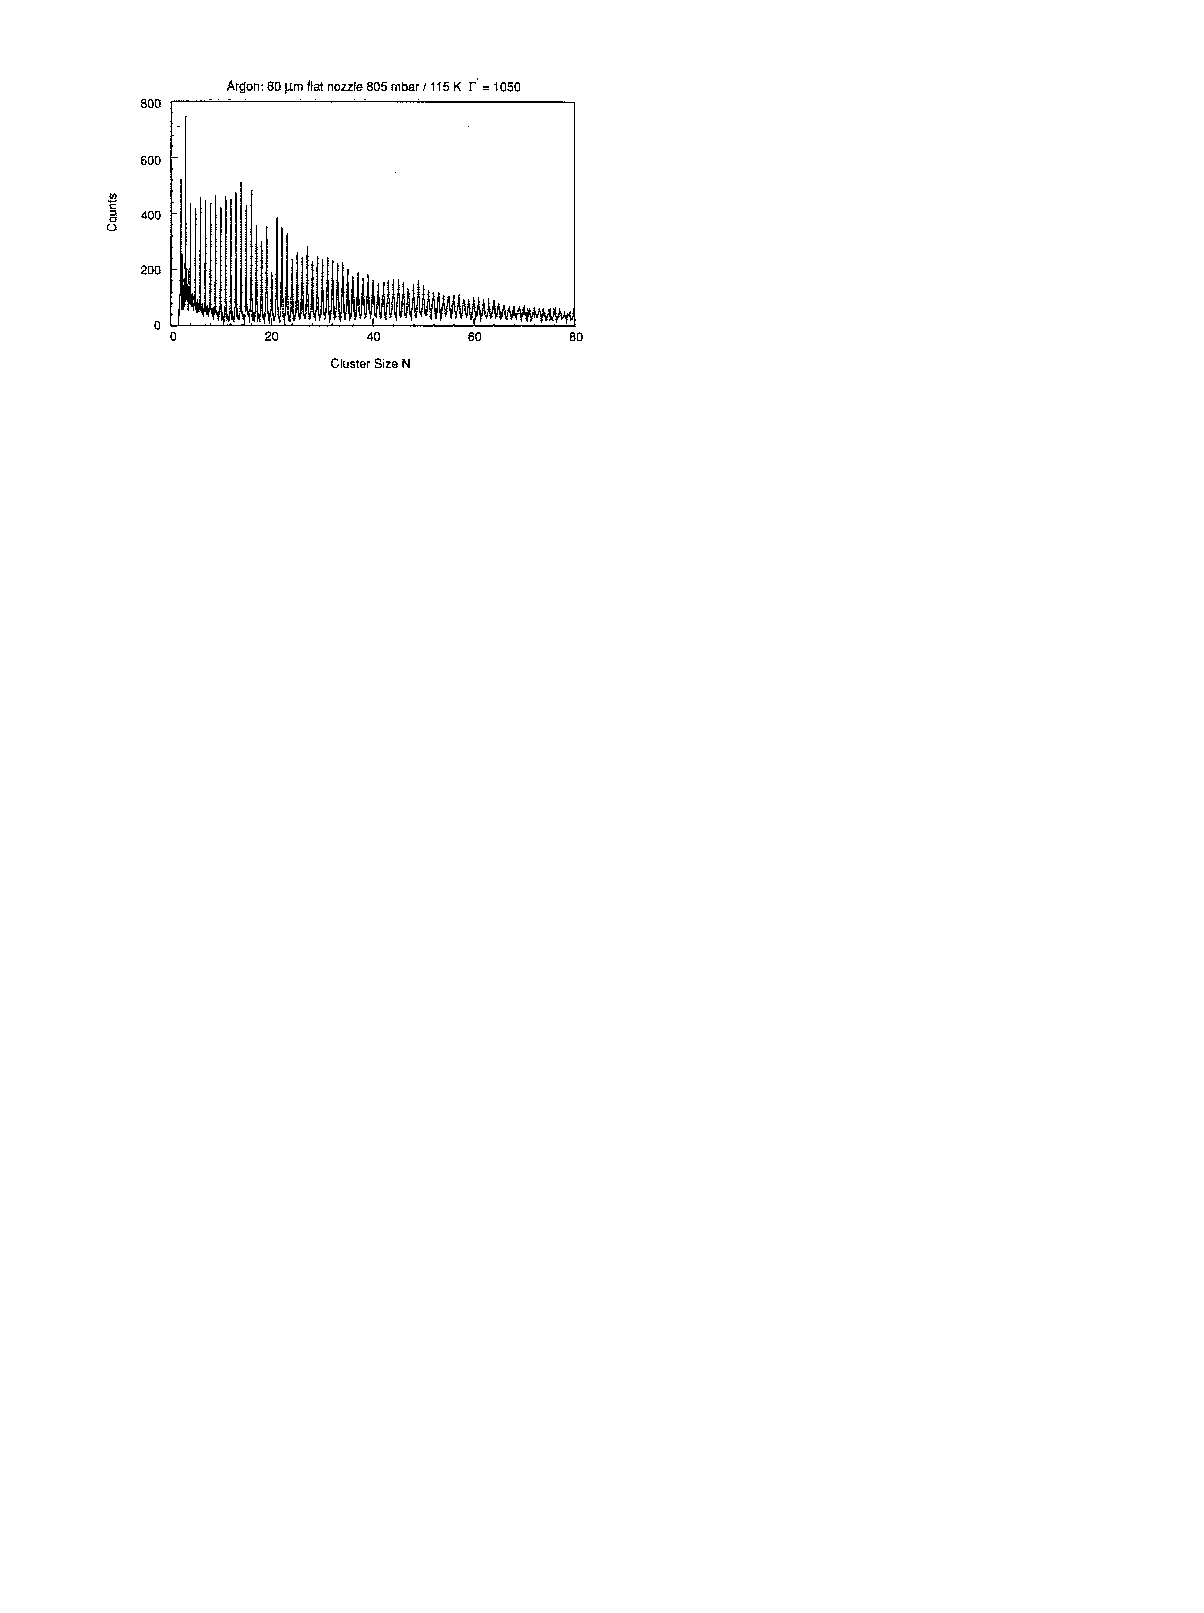
\includegraphics[scale=1.0]{pics/exp_clusters1.pdf}
  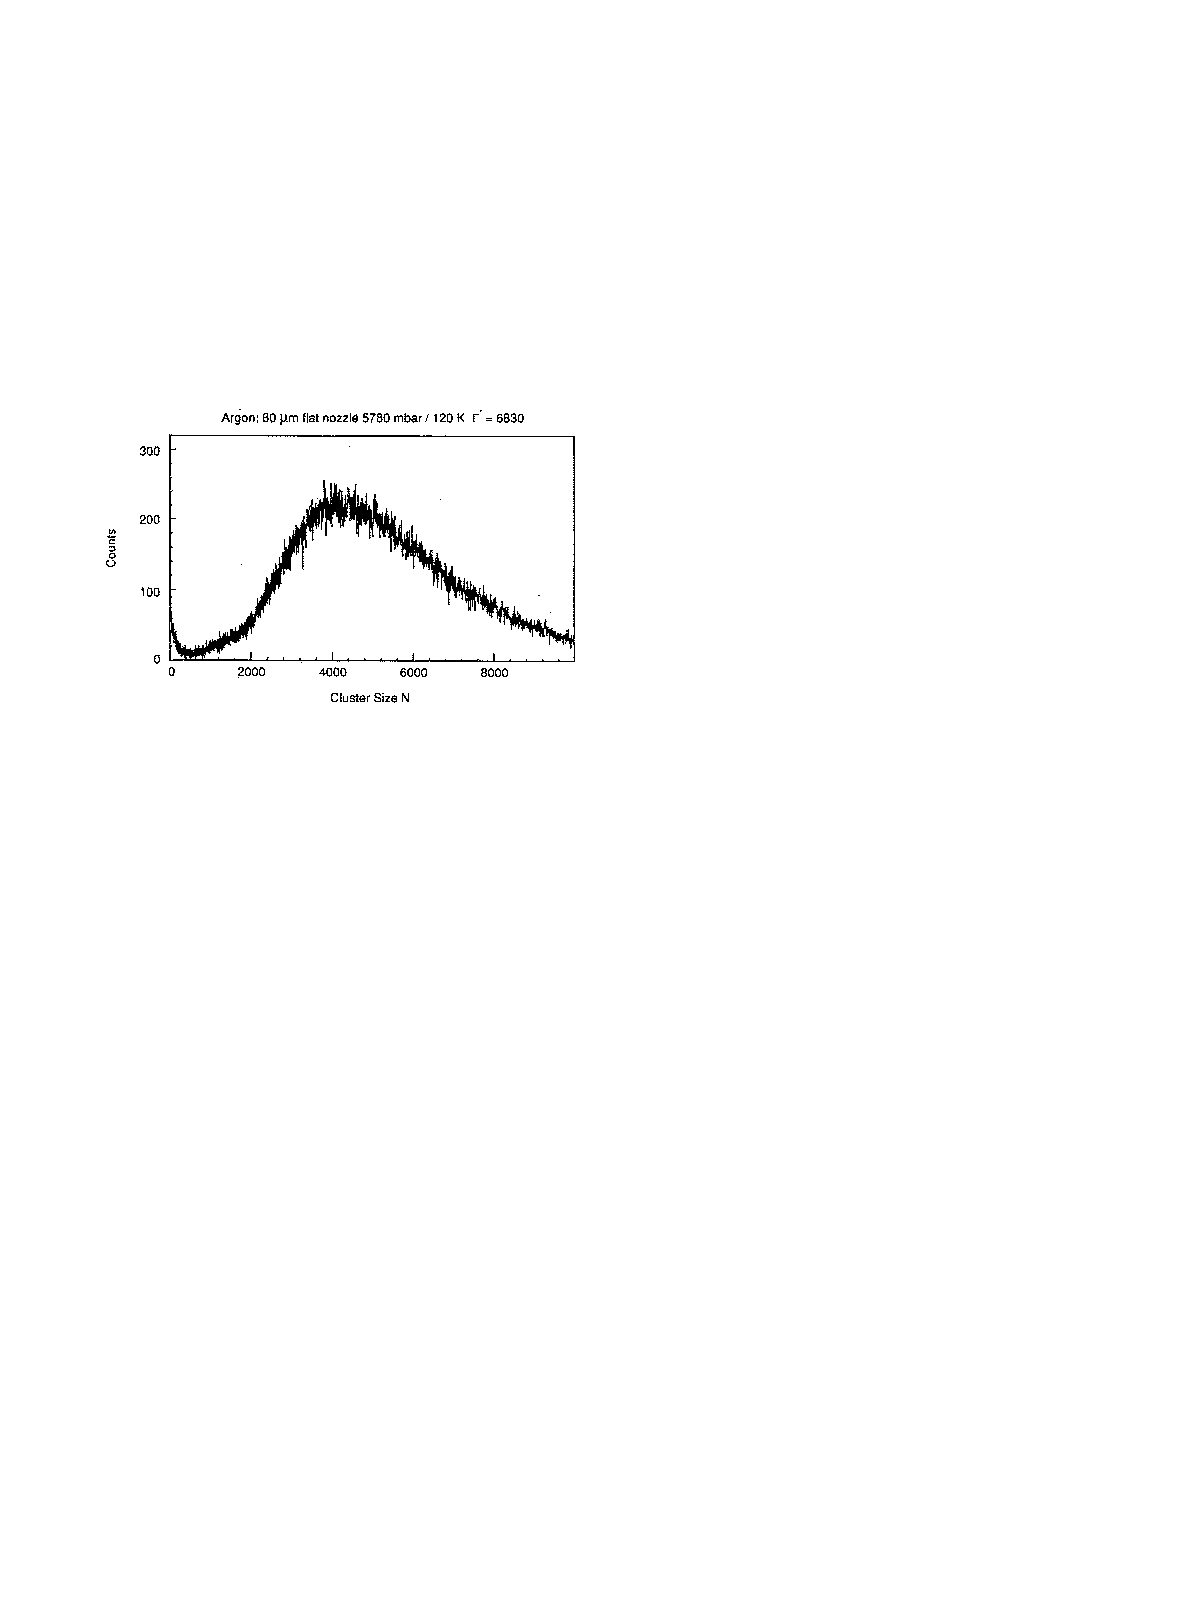
\includegraphics[scale=1.0]{pics/exp_clusters2.pdf}
  \caption{Mass distribution of argon clusters. Reprint with permission
           from Ref. \cite{Karnbach93}. Copyright 1993, AIP Publishing LLC.}
  \label{figure:cluster_mass}
\end{figure}

The mean cluster size $\bar{N}$ can be estimated with
the help of the empirical scaling parameter $\Gamma^*$ of Hagena \textit{et al.}
\cite{Hagena72,Hagena81} for different experimental conditions.

\begin{equation}
 \Gamma^* = \frac{p_0 d_{eq}^q}{T_0^{5/2-q/4}} K_{ch}
\end{equation}
Here, $p_0$ and $T_0$ are the expansion pressure and the temperature
of the nozzle and $d_{eq}$ is the equivalent nozzle diameter for conical
nozzles. $K_{ch}$ is a constant depending on the material and can be
calculated by the means of Hagena \cite{Hagena87}. The values for the rare gases for
the experimental setup, which will be compared to in this work are
$K_{ch}(Ne)=185$, $K_{ch}(Ar)=1646$, $K_{ch}(Kr)=2980$ and $K_{ch}(Xe)=5554$
\cite{PhDFoerstel}.

From the scaling parameter the mean cluster size $\bar{N}$ 
of homonuclear clusters can be
estimated as

\begin{equation}
  \bar{N} = 33 \left( \frac{\Gamma^*}{1000} \right) ^{2.35} .
\end{equation}


\subsection{Creation of Heteronuclear Noble Gas Clusters}
Heteronuclear noble gas clusters can be created in different ways:
the \emph{pick-up} method or co-expansion of two different gases are two examples.
For the pick-up method, the jet of homonuclear clusters is directed through
a volume with a high concentration of the other species. The clusters
collide with the second species of which consequently atoms or molecules
are attached to the surface
of the parent cluster. Depending on the species
and the experimental conditions, different cluster arrangements can be observed.
Either, few atoms
of the second species stay on the surface of the parent cluster,
several atoms form a shell around the parent cluster or the second species
diffuses into the bulk of the parent cluster.

In the co-expansion method two gases are mixed before the expansion and
then led into the nozzle together. The species with the higher cohesive
energy is more likely to start nucleation and form dimers which
then grow into larger clusters.



\section{Experimental Analysis Tools}
Noble gas clusters are investigated using mass spectrometry and spectroscopy.
From the mass spectrometry information about the mean number of atoms
can be obtained. Within spectroscopy two ansatzes are used
to gain information about clusters. In the first one, measurements of
atomic properties for atoms in clusters are compared to the results of
atoms. From the number of peaks, the energy shift and the relative peak
intensity conclusions about the surroundings about the atoms inside
the cluster are drawn. These methods are \ac{PES}, especially \ac{XPS}
and \ac{UPS}, \ac{AES}, \ac{RAS}, \ac{XES}, \ac{NEXAFS} and \ac{XAS}.
Their different working principles are illustrated in Figure
\ref{figure:overview_spectroscopies}.

\begin{figure}[h]
  \centering
  \begin{tikzpicture}[
          scale=1.0,>=stealth
        ]
%     \tiny
 % \draw[very thin,color=gray] (-0.1,-4.1) grid (10.9,4.9);
 \draw [->, thick] (0,0) -- (0,6) node [left]{$E$};
 \tiny
 \draw (1,0.5) node[left]{Core}  -- (2,0.5);
 \fill [diplom1] (1.25,0.5) circle (0.07);
 \fill [diplom1] (1.75,0.5) circle (0.07);
 \draw (1,0.7) node[left]{Valence} -- (2,0.7) node[right]{Ground state};
 \fill [diplom1] (1.25,0.7) circle (0.07);
 \fill [diplom1] (1.75,0.7) circle (0.07);
 \draw[dashed] (1,0.9) -- (2,0.9);

\begin{scope}[yshift=3cm]
 \draw (1,0.5) -- (2,0.5);
 \fill [diplom1] (1.25,0.5) circle (0.07);
 \draw (1,0.7)  -- (2,0.7) node[right, align=center]{Core-excited\\state};
 \fill [diplom1] (1.25,0.7) circle (0.07);
 \fill [diplom1] (1.75,0.7) circle (0.07);
 \draw[dashed] (1,0.9) -- (2,0.9);
 \fill [diplom1] (1.75,0.9) circle (0.07);
\end{scope}

\begin{scope}[xshift=3cm,yshift=4cm]
 \draw (1,0.5) -- (2,0.5);
 \fill [diplom1] (1.25,0.5) circle (0.07);
 \draw (1,0.7)  -- (2,0.7) node[right, align=center]{Core-ionized\\state};
 \fill [diplom1] (1.25,0.7) circle (0.07);
 \fill [diplom1] (1.75,0.7) circle (0.07);
 \draw[dashed] (1,0.9) -- (2,0.9);
\end{scope}

\begin{scope}[xshift=3cm,yshift=1cm]
 \draw (1,0.5) -- (2,0.5);
 \fill [diplom1] (1.25,0.5) circle (0.07);
 \fill [diplom1] (1.75,0.5) circle (0.07);
 \draw (1,0.7)  -- (2,0.7) node[right, align=center]{Valence-ionized\\state};
 \fill [diplom1] (1.75,0.7) circle (0.07);
 \draw[dashed] (1,0.9) -- (2,0.9);
\end{scope}

\begin{scope}[xshift=6cm,yshift=1.7cm]
 \draw (1,0.5) -- (2,0.5);
 \fill [diplom1] (1.25,0.5) circle (0.07);
 \fill [diplom1] (1.75,0.5) circle (0.07);
 \draw (1,0.7)  -- (2,0.7) node[right, align=center]{Doubly valence-\\ionized state};
 \draw[dashed] (1,0.9) -- (2,0.9);
\end{scope}

\coordinate (GS) at (1.7,0.95);
\coordinate (CES) at (1.7,3.30);
\coordinate (CIS) at (4.5,4.00);
\coordinate (VIS) at (4.5,2.00);
\coordinate (DVIS) at (6.5,2.50);

\draw [thick,diplom2,->] (GS) -- (CES);
\node [fill=white] at ($ (GS)!0.5!(CES) $) {\color{diplom2}NEXAFS / XAS};

\draw [thick,diplom2,->] (GS) -- (CIS);
\node [fill=white] at ($ (GS)!0.5!(CIS) $) {\color{diplom2}XPS};
 
\draw [thick,diplom2,->] (GS) -- (VIS);
\node [fill=white] at ($ (GS)!0.5!(VIS) $) {\color{diplom2}UPS};
 
\draw [thick,diplom2,->] (CIS) -- (VIS);
\node [fill=white] at ($ (CIS)!0.5!(VIS) $) {\color{diplom2}XES};
 
\draw [thick,diplom2,->] (CIS) -- (DVIS);
\node [fill=white] at ($ (CIS)!0.5!(DVIS) $) {\color{diplom2}AES};
 
\end{tikzpicture}

  \caption{Schematic overview over the physical mechanisms of different
           spectroscopic methods \cite{Bjorneholm09}.}
  \label{figure:overview_spectroscopies}
\end{figure}

\ac{XAS}, also known as \ac{NEXAFS} probe the absorption of light
from the ground state to a core excited state With \ac{PES} ionization
energies can be determined. More accurately \ac{UPS} gives information
about the ionization potentials of valence orbitals and \ac{XPS}
of core orbitals.
\ac{AES} measures the kinetic energy of the emitted Auger electron
resulting in a doubly (mostly valence) ionized final state, while
\ac{XES} measures the photon emitted during an relaxation from
a core ionized to valence ionized state.

Using thoses techniques, atoms in the bulk can be differentiated from atoms
in the surface and even different positions in the
outermost shell could be resolved. The obtained surface-to-bulk ratios
can then also be used for an estimation of the mean cluster size
\cite{Bjorneholm09,Knop98,Hatsui05}.

The second ansatz, which is developed in this thesis, uses electron-electron
and ion-ion coincidence spectroscopy.
They exploit the interaction between neighbouring atoms
directly using the ICD.
Until now, these techniques
have been used for the investigation of the
\ac{ICD} and \ac{ICD}-like processes alone.
But since the ICD-like processes strongly depend on the geometry, I am going to
show that for systems with two competitive processes of comparable lifetime,
having information about the decay widths, conclusions about
the cluster structure can be drawn with the help of experimental
electron-electron spectra.

\begin{figure}[h]
  \centering
  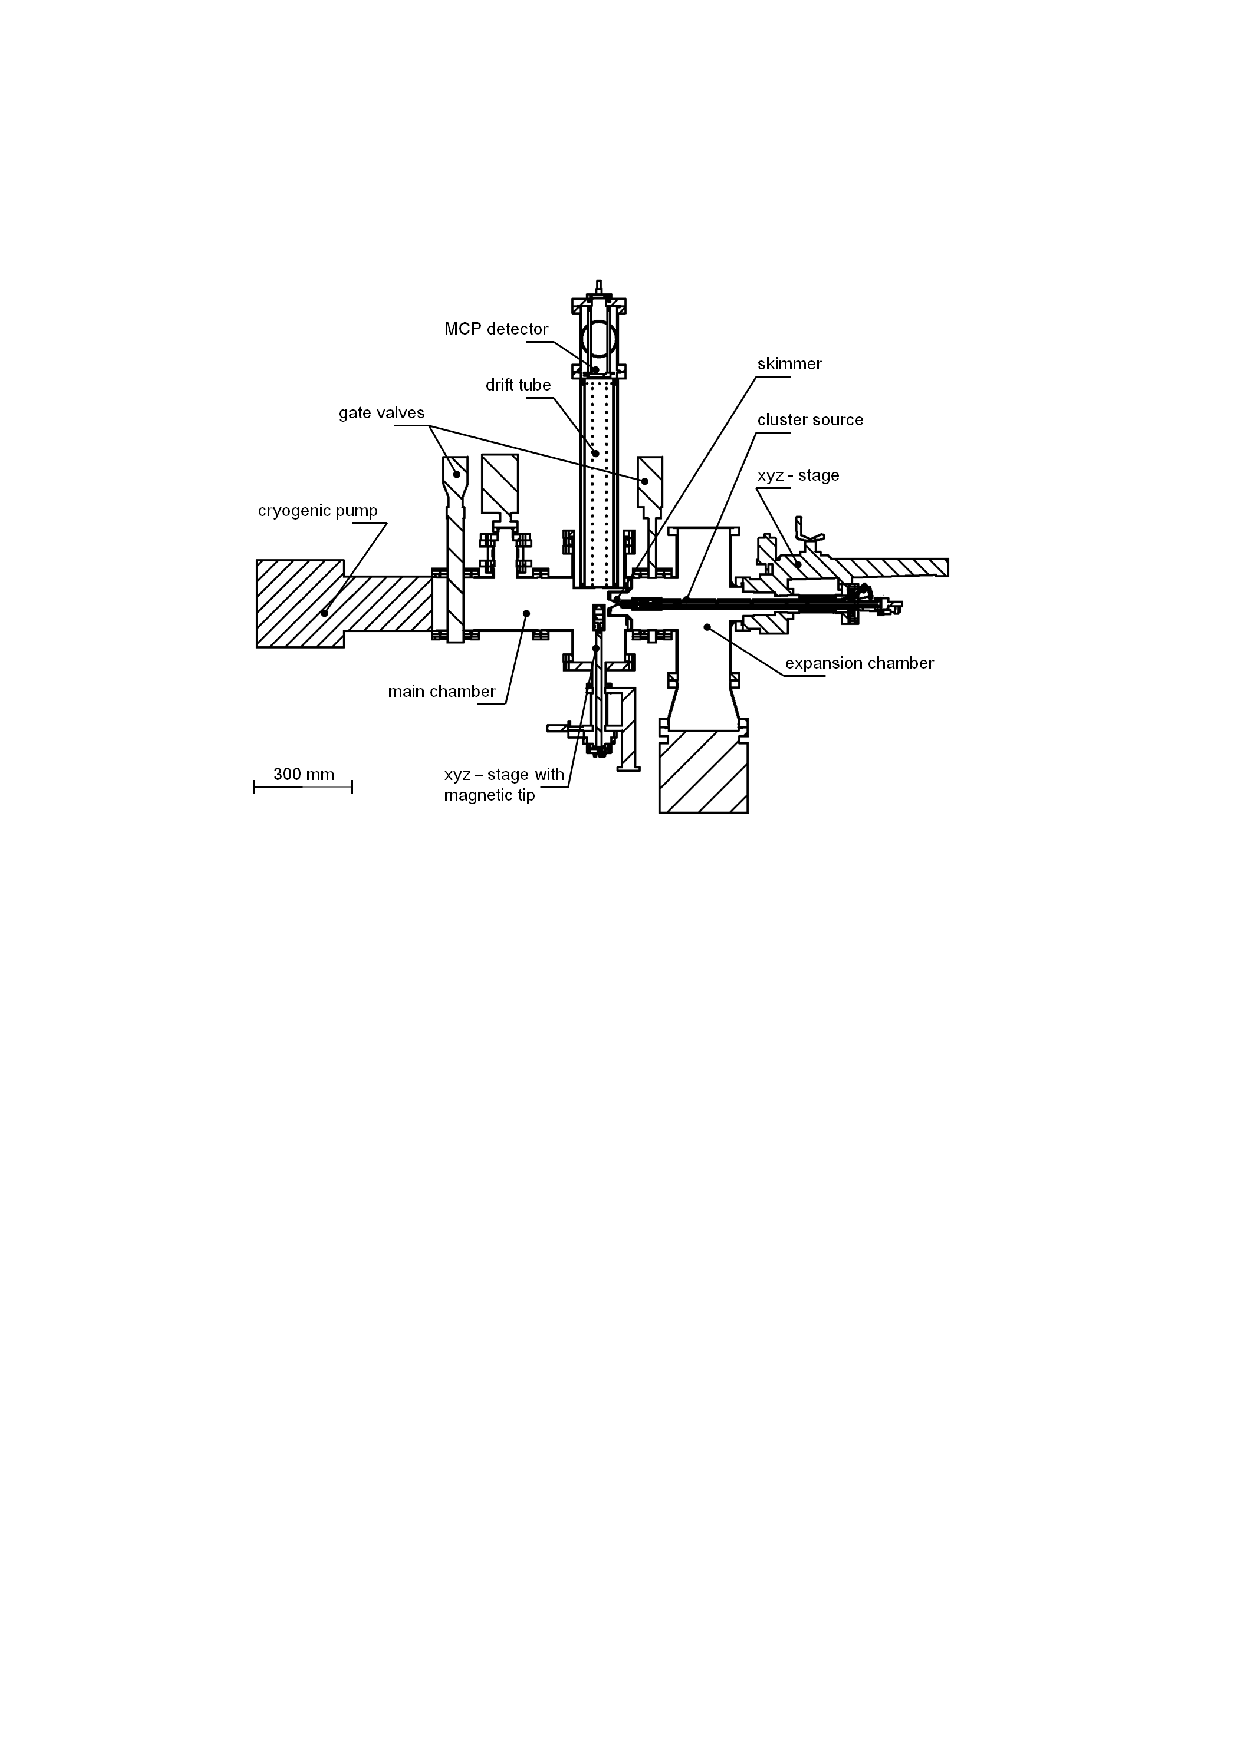
\includegraphics[]{pics/exp_setup_overview.pdf}
  \caption{Schematic view of the experimental setup of a electron-electron
           coincidence measurement. The synchrotron radiation axis
           is perpendicular to the plane of the diagram.
           Reprinted with permission from \cite{PhDFoerstel}. }
  \label{figure:exp_setup_overview}
\end{figure}

The principle experimental setup for both coincidence measurements is very similar.
As shown in Figure \ref{figure:exp_setup_overview},
the clusters are created using supersonic expansion into
the expansion chamber. The jet is then directed through a conical skimmer
into the reaction chamber. Here, 
the jet is crossed with synchrotron radiation.
One pulse has of course many many photons. However, only 1 in about 10000
pulses creates a vacancy.
This created vacancy can then decay via ICD.
In this case, a second electron is emitted and the two positively charged
subsystems undergo
Coulomb explosion within a timescale of \unit{fs} to \unit[]{ps}.
In this time scale, the ionized cluster is still inside the reaction sphere.
Initiated by the synchrotron photon, four charged particles are created,
two electrons and two ions.
Being charged, these particles can easily be withdrawn from the reaction
chamber to detectors using a so-called magnetic bottle for both positively
and negatively charged particles. In experiments normally only either electrons
or ions are investigated at a time.

A coincidence of two particles is experimentally defined by two events
measured in a specific time range after one synchrotron pulse.
For the
electron-electron coincidence, the coincidence time range is \unit[1600]{ns}
\cite{Foerstel_private}.
Coincidences are very often displayed in a so-called coincidence map,
where the kinetic energy of one electron is plotted against the
kinetic energy of the other electron. 
Two electrons measured in coincidence can stem from several physical
processes. In the coincidence map these processes are distinguishable
from the form of the signal.

\begin{figure}[h]
  \centering
  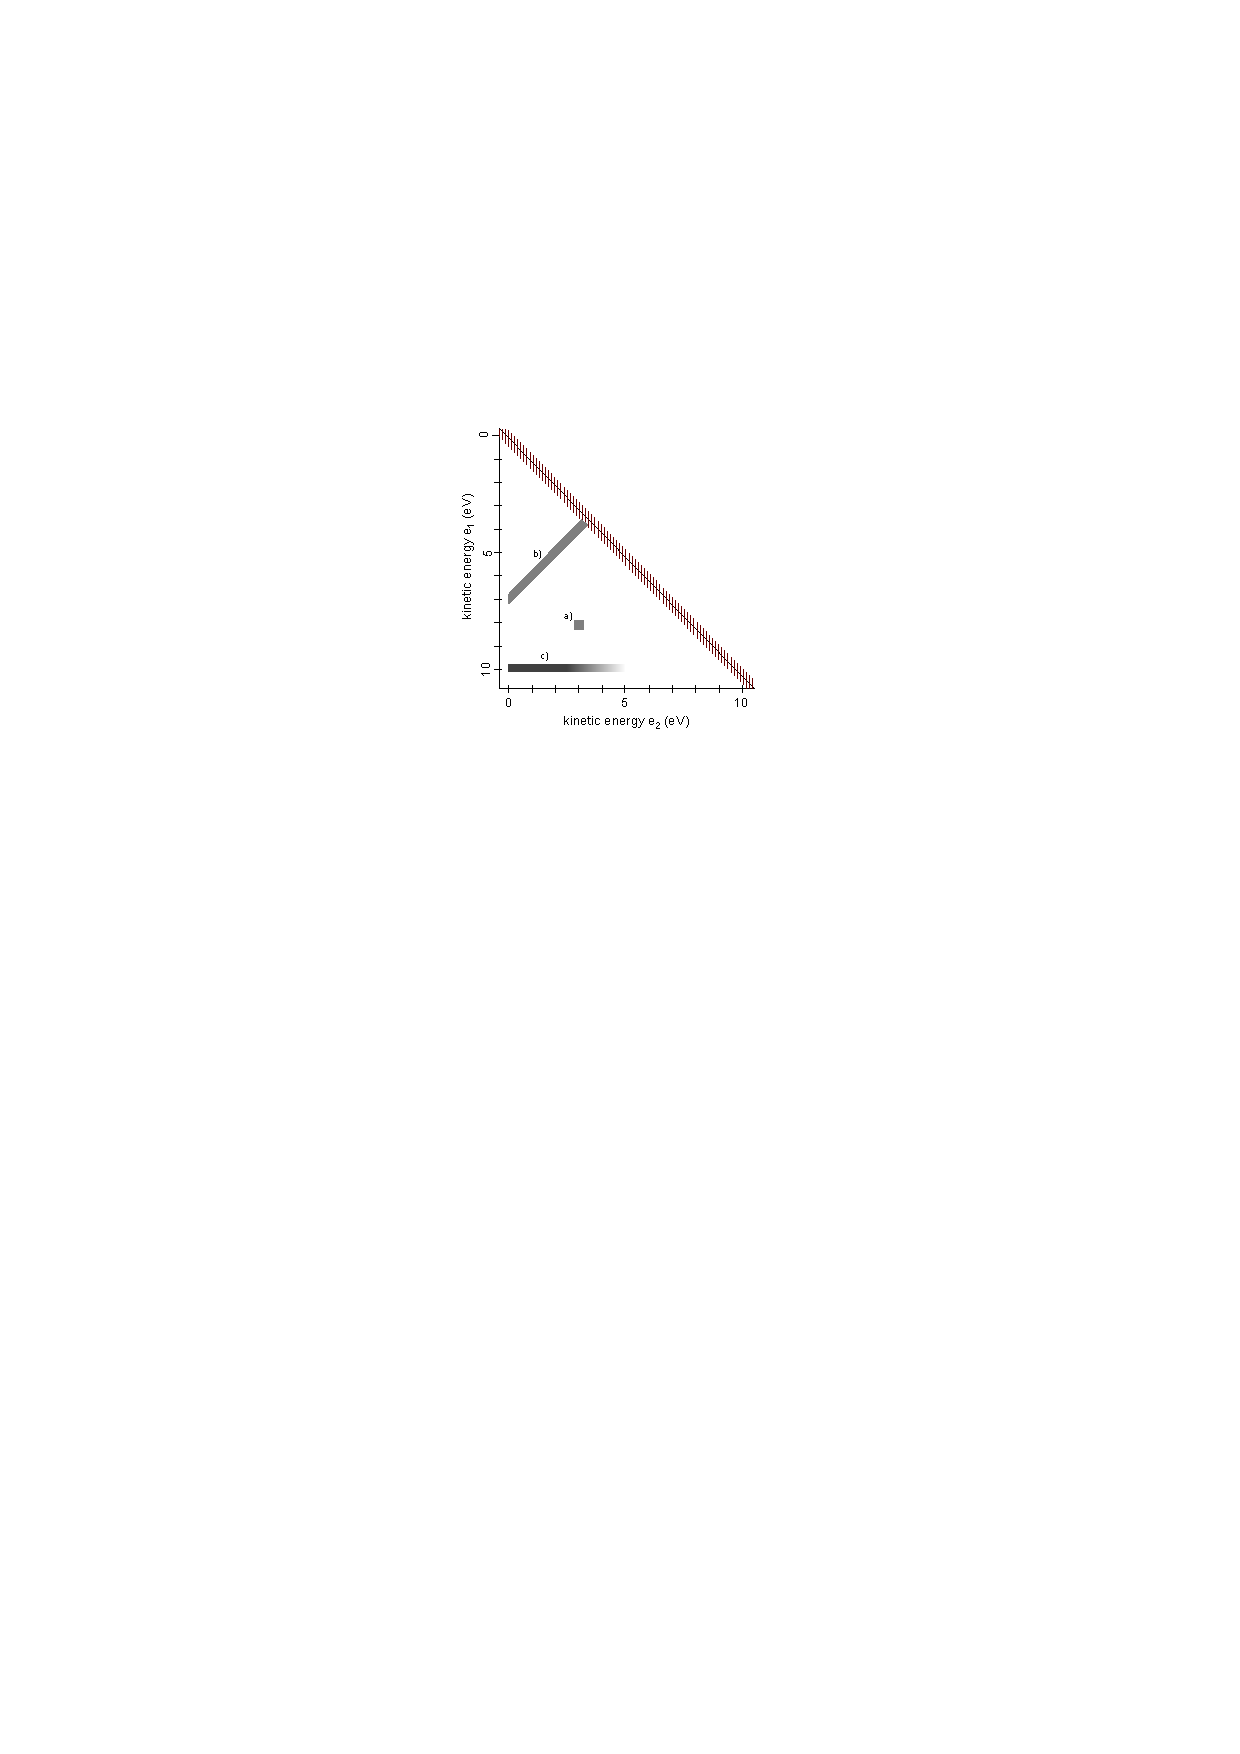
\includegraphics{pics/ee_coincidence_processes.pdf}
  \caption{Schematic illustration of electron-electron
           coincidence signatures for different physical processes.
           \cite{PhDFoerstel} See the text for details.}
  \label{figure:ee_coincidence_processes}
\end{figure}

Figure \ref{figure:ee_coincidence_processes} illustrates such a coincidence
map. There, the signal a) is a spot at defined energies $e_1$ and $e_2$.
It corresponds to a process, where the electrons both stem from orbitals
of a well defined, small energy range and the final state energy is not
influenced by perturbations like vibrations. This could e.g. be an Auger
decay.
Signal b) is a straight line with a constant sum of the kinetic electron
energies. For example electron-electron scattering shows such a behaviour.
Signal c) is a smeared out line, where one electron energy is constant
and the kinetic energy of the second electron underlies a distribution.
An ICD process would exhibit such a signal. Here the ionization energy
for the creation of the initial state is quite well defined, whereas
the energy of the final states shows a broad distribution due to
vibrations and, as is to be shown in this thesis, due to several decay
channels with different final state energies as well as a decay involving
atoms at different distances inside larger clusters.

To visualize the coincident data and especially the ICD feature one can
extract and plot only those electrons which are detected in coincidence with
electrons from the initially excited, autoionizing state.
The histogrammized counts of these electrons over their kinetic energy is
then the coincidence spectrum.
spectrum. An example  of a coinicident electron spectrum is shown in Figure
Figure \ref{figure:ICD_spectrum_example}. Two distinct features can be
seen which are detected in coincidence with a Ne2s electron. They correspond
to the two competing processes of NeNe-ICD and NeAr-ICD, which will be
discussed in detail in chapter \ref{chapter:NeArclusters}.


\begin{figure}[h]
  \centering
  \includegraphics{pics/exp_near_coinc_sets.eps}
  \caption{Electron-electron coincidence spectra for NeAr clusters
           showing both NeNe-ICD and NeAr-ICD signals \cite{Fasshauer14_1}.}
  \label{figure:ICD_spectrum_example}
\end{figure}
